\documentclass[12pt]{article}
\usepackage{natbib}
\usepackage{url}
\usepackage{stmaryrd}
\usepackage{mathrsfs}
\usepackage{amsmath}
\usepackage{graphicx}
\usepackage{parskip}
\usepackage{fancyhdr}
\usepackage{commath}%定义d
\usepackage[UTF8,scheme = plain]{ctex}
\usepackage{geometry}
\usepackage{bm}
\usepackage{siunitx}
\usepackage{float}
\usepackage{subfig}
\usepackage{titlesec}
\usepackage{caption}
\usepackage{paralist}
\usepackage{multirow}
\usepackage{booktabs} % To thicken table lines
\usepackage{diagbox}
\usepackage{authblk}
\usepackage{indentfirst}
\usepackage{amsthm}
\usepackage{fontspec}
\usepackage{color}
%\usepackage{txfonts} %设置字体为times new roman
\usepackage{lettrine}
\usepackage{nameref}
%\usepackage[nottoc]{tocbibind}
\usepackage{amssymb}%font
\usepackage{lipsum}%make test words
\usepackage{picinpar}%words around the picture
\usepackage[all]{xy}%draw arrow
\usepackage{asymptote}%draw picture
\usepackage[perpage]{footmisc}%脚注每页清零
\usepackage{esint}

\geometry{bottom=3cm,left=3cm,right=3cm,top=3cm}
% \footskip = 60pt

% \setmainfont{TimesNewRomanPSMT}
\setsansfont{Helvetica-Light}
\setCJKmainfont[ItalicFont=STKaitiSC-Regular,BoldFont=STSongti-SC-Black]{STSongti-SC-Regular}
\setCJKsansfont[BoldFont=STHeitiSC-Medium]{STHeitiSC-Light}


%\setmainfont{Times New Roman}

\ctexset{today=old}%日期类型设置

% ======================================
% = Color de la Universidad de Sevilla =
% ======================================
\usepackage{tikz}
\definecolor{PKUred}{cmyk}{0,1,1,0.45}

%超链接设置
\usepackage[breaklinks,colorlinks,linkcolor=PKUred,citecolor=PKUred,pagebackref,urlcolor=PKUred]{hyperref}
\usepackage{cleveref}
% \newcommand{\crefpairconjunction}{ 和 }


\newcommand{\hsp}{\hspace{20pt}}
\newcommand{\nhsp}{\hspace{-30pt}}
\titleformat{\section}{\Large\bfseries}{%\arabic{section}
\hspace{-22pt}\textcolor{PKUred}{\vrule width 2pt}\hsp}{0pt}{}


\titleformat{\subsection}
  {\normalfont\large\bfseries}{}{0em}{}

\renewcommand*\footnoterule{%
    \vspace*{-3pt}%
    {\color{PKUred}\hrule width 2in height 0.4pt}%
    \vspace*{2.6pt}%
}


%% Color the bullets of the itemize environment and make the symbol of the third
%% level a diamond instead of an asterisk.
%h\renewcommand*\textbullet{\dag}
\renewcommand*\labelitemi{\color{PKUred}\textbullet}
\renewcommand*\labelitemii{\color{PKUred}--}
\renewcommand*\labelitemiii{\color{PKUred}$\diamond$}
\renewcommand*\labelitemiv{\color{PKUred}\textperiodcentered}



%%% Equation and float numbering
\numberwithin{equation}{section}		% Equationnumbering: section.eq#
\numberwithin{figure}{section}			% Figurenumbering: section.fig#
\numberwithin{table}{section}				% Tablenumbering: section.tab#


%代码设置
\usepackage{listings}
\usepackage{fontspec} % 定制字体
\newfontfamily\menlo{SFMono-Regular}
\usepackage{xcolor} % 定制颜色
\definecolor{mygreen}{rgb}{0,0.6,0}
\definecolor{mygray}{rgb}{0.5,0.5,0.5}
\definecolor{mymauve}{rgb}{0.58,0,0.82}
\lstset{  
numbers=left,
numberstyle=\footnotesize\menlo,
basicstyle=\footnotesize\menlo,
backgroundcolor=\color{white},      % choose the background color
columns=fullflexible,
tabsize=4,
breaklines=true,               % automatic line breaking only at whitespace
captionpos=b,                  % sets the caption-position to bottom
commentstyle=\color{mygreen},  % comment style
escapeinside={\%*}{*)},        % if you want to add LaTeX within your code
keywordstyle=\color{blue},     % keyword style
stringstyle=\color{mymauve}\ttfamily,  % string literal style
frame=single,
rulesepcolor=\color{red!20!green!20!blue!20},
% identifierstyle=\color{red},
language=c++,
xleftmargin=4em,xrightmargin=2em, aboveskip=1em,
framexleftmargin=2em,
numbers=left
}

%脚注
\renewcommand\thefootnote{\fnsymbol{footnote}}

%定义常数i、e、积分符号d
\newcommand\mi{\mathrm{i}}
\newcommand\me{\mathrm{e}}

%%% Maketitle metadata
\newcommand{\horrule}[1]{\rule{\linewidth}{#1}} 	% Horizontal rule
\newcommand{\tabincell}[2]{\begin{tabular}{@{}#1@{}}#2\end{tabular}}


\setcounter{secnumdepth}{2}
\usepackage{bm}
\usepackage{autobreak}
\usepackage{amsmath}
\graphicspath{{fig/}}
\setlength{\parindent}{2em}

%pdf文件设置
\hypersetup{
	pdfauthor={袁磊祺},
	pdftitle={Advanced Fluid Mechanics Homework 2}
}

\title{
		\vspace{-1in} 	
		\usefont{OT1}{bch}{b}{n}
		\normalfont \normalsize \textsc{\LARGE Peking University}\\[1cm] % Name of your university/college \\ [25pt]
		\horrule{0.5pt} \\[0.5cm]
		\huge \bfseries{Advanced Fluid Mechanics Homework 2} \\
		\horrule{2pt} \\[0.5cm]
}
\author{
		\normalfont 								\normalsize
		College of Engineering \quad 2001111690  \quad 袁磊祺\\	\normalsize
        \today
}
\date{}

\begin{document}

%%%%%%%%%%%%%%%%%%%%%%%%%%%%%%%%%%%%%%%%%%%%%%
\captionsetup[figure]{name={图},labelsep=period}
\captionsetup[table]{name={表},labelsep=period}
\renewcommand\contentsname{目录}
\renewcommand\listfigurename{插图目录}
\renewcommand\listtablename{表格目录}
\renewcommand\refname{参考文献}
\renewcommand\indexname{索引}
\renewcommand\figurename{图}
\renewcommand\tablename{表}
\renewcommand\abstractname{摘\quad 要}
\renewcommand\partname{部分}
\renewcommand\appendixname{附录}
\def\equationautorefname{式}%
\def\footnoteautorefname{脚注}%
\def\itemautorefname{项}%
\def\figureautorefname{图}%
\def\tableautorefname{表}%
\def\partautorefname{篇}%
\def\appendixautorefname{附录}%
\def\chapterautorefname{章}%
\def\sectionautorefname{节}%
\def\subsectionautorefname{小小节}%
\def\subsubsectionautorefname{subsubsection}%
\def\paragraphautorefname{段落}%
\def\subparagraphautorefname{子段落}%
\def\FancyVerbLineautorefname{行}%
\def\theoremautorefname{定理}%
\crefname{figure}{图}{图}
\crefname{equation}{式}{式}
\crefname{table}{表}{表}
%%%%%%%%%%%%%%%%%%%%%%%%%%%%%%%%%%%%%%%%%%%

\maketitle

\section{1}



已知来流速度为$U$, 下截面速度分布为$u(y)$, 单位长度物体受到的阻力为$\vec{D}$

取一个静止的闭曲面,上下水平延伸到无穷远,左右竖直延伸到无穷远。因为是定常流动,面内的总动量保持不变
\begin{equation}
	\pd{}{t} \iiint \rho \vec{u} \dif V = - \oiint \rho \vec{u} u_n \dif S - \vec{D} - \oiint p \vec{n} \dif S = 0,
\end{equation}
\begin{equation}
	\vec{D} = - \oiint \rho \vec{u} u_n \dif S - \oiint p \vec{n} \dif S.
\end{equation}
伯努利方程
\begin{equation}
	p + \frac{\rho}{2} u^2 = p_{\infty} + \frac{\rho}{2} U^2.
\end{equation}
所以
\begin{equation}
	\begin{aligned}
		D = & - \oiint \rho \vec{u} u_n \dif S - \oiint p \vec{n} \dif S\\
		= & - \int_{-\infty}^{\infty} \rho \vec{u} u_n \dif l - \int_{-\infty}^{\infty} p \vec{n} \dif l\\
		= & - \int_{-\infty}^{\infty} \frac{\rho}{2} \left(u^2 - U^2\right) \dif l + \int_{-\infty}^{\infty} \rho \left(u^2 - U^2\right) \dif l\\
		= & - \frac{\rho}{2} \int_{-\infty}^{\infty} (U+u)(U-u) \dif l\\
		\approx & - \rho \int_{-\infty}^{+\infty} U(U-u) \dif y.
	\end{aligned}
\end{equation}
其中$\rho$是流体的密度,这里用到了$u\approx U$的近似.

\begin{figure}[htp]
	\centering
	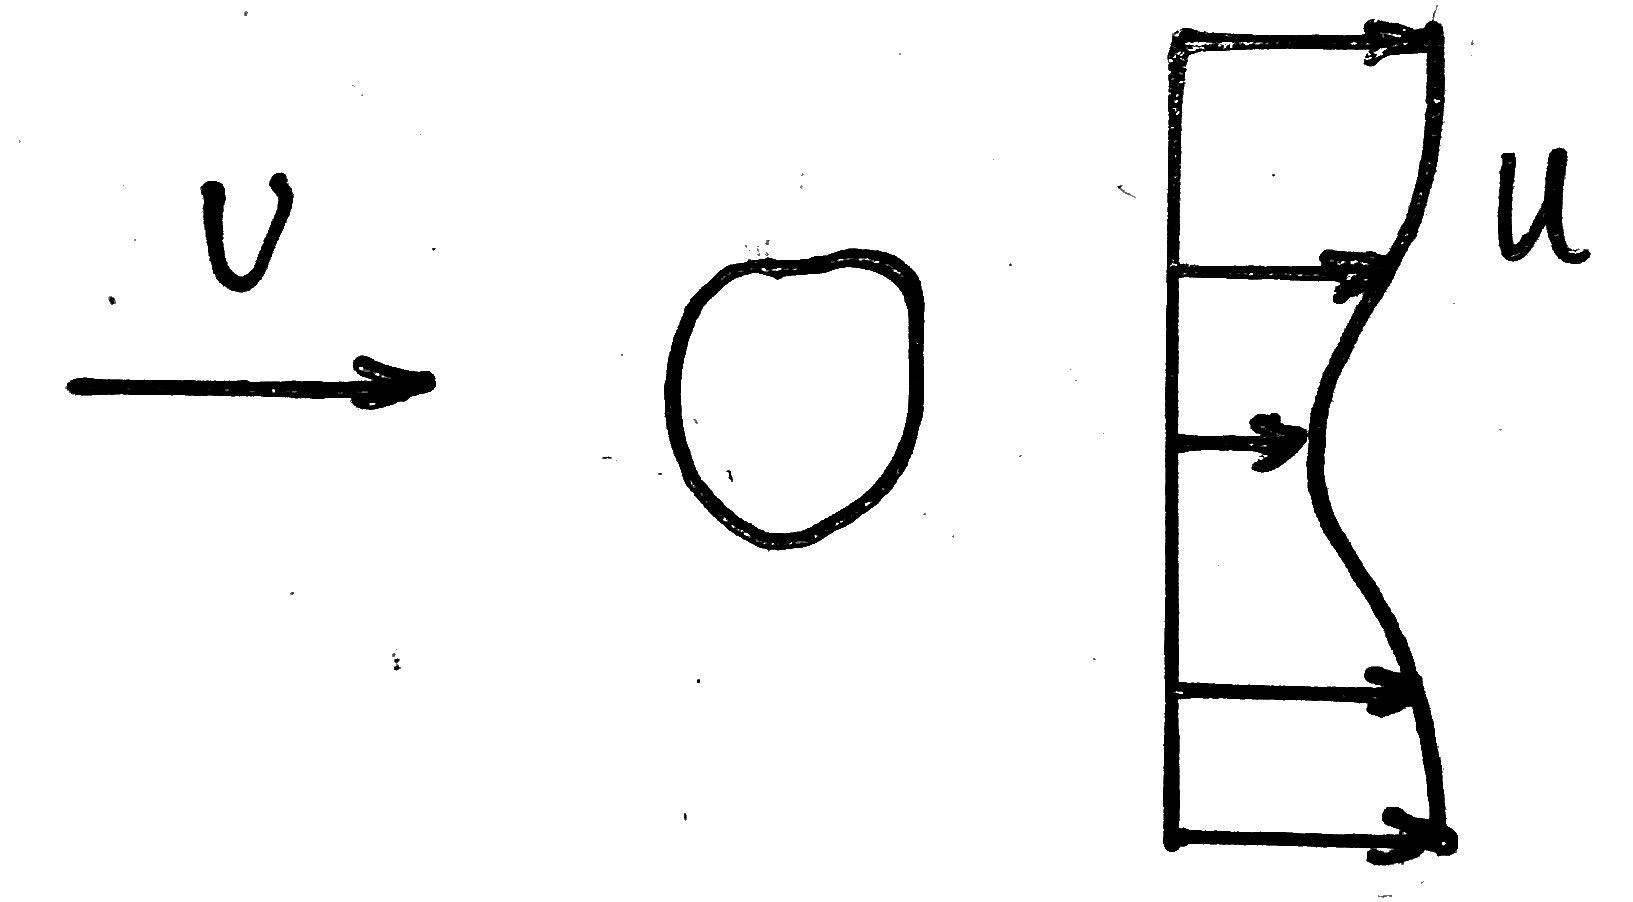
\includegraphics[width=8cm]{1.jpeg}
	\caption{二元风洞或水洞中测量钝体绕流尾流下游截面上速度分布}
	\label{fig:1}
\end{figure}


\section{2}

Assume the flow at a sufficiently larger fixed control surface Σ is irrotational, the pressure can be replaced by $−\abs{\bm{u}}^2/2$ due to the Bernoulli integral:
\begin{equation}
	\boldsymbol{F}=\rho \int_{\Sigma}\left(\frac{1}{2}|\boldsymbol{u}|^{2} \boldsymbol{n}-\boldsymbol{u} \boldsymbol{u} \cdot \boldsymbol{n}\right) d S
\end{equation}
Let $\bm{u} = \bm{U} + \bm{v}$ with $\bm{v}$ being the disturbance velocity that approaches zero at infinity, such that
\begin{equation}
	\begin{aligned}
	\frac{1}{2}|\boldsymbol{u}|^{2} n_{i}-u_{i} u_{j} n_{j}=& \frac{1}{2}|v|^{2} n_{i}+U_{j} v_{j} n_{i}+\frac{1}{2} U^{2} n_{i} \\
	&-v_{i} v_{j} n_{j}-U_{i} v_{j} n_{j}-v_{i} U_{j} n_{j}-U_{i} U_{j} n_{j}.
	\end{aligned}
\end{equation}

For two-dimensional flow
\begin{equation}
	\int_{\Sigma} \boldsymbol{n} \times \boldsymbol{v} d S=\int_{V} \boldsymbol{\omega} d V=\boldsymbol{e}_{z} \Gamma.
\end{equation}

So,
\begin{equation}
	\boldsymbol{F}=-\rho U \Gamma \bm{e}_{y}.
\end{equation}

\section{3}

\subsection{非零下界}

速度分解为
\begin{equation}
	\bm{u} = \nabla \phi + \nabla \times \Psi.
\end{equation}

因为有不可压缩条件
\begin{equation}
	\nabla \cdot \bm{u} = 0,
\end{equation}
所以
\begin{equation}
	\Delta \phi =  0.
	\label{eq:3.1}
\end{equation}

计算拟涡能
\begin{equation}
	\iiint \frac{1}{2} \omega^2 \dif V = \iiint \frac{1}{2} \nabla \times (\nabla \times \Psi) \cdot  \nabla \times (\nabla \times \Psi)  \dif V = \iiint \frac{1}{2} (\Delta \Psi) \cdot (\Delta \Psi) \dif V.
\end{equation}
如果拟涡能等于0, 则
\begin{equation}
	\Delta \Psi = 0.
	\label{eq:3.2}
\end{equation}
由\cref{eq:3.1,eq:3.2} 解得的方程很可能无法边界条件, 所以拟涡能有一个非零下界.

\subsection{}

旋转部件?




\section{4}

多连通区域并不影响泊松方程的求解, 所以Helmholtz-Hodeg分解定理保持不变.

\begin{equation}
	\bm{u} = \nabla \phi + \nabla \times \Psi,
\end{equation}
\begin{equation}
	\nabla \cdot \Psi = 0.
\end{equation}

\section{5}

\subsection{无界流场}

在无界流场求解拉普拉斯方程
\begin{equation}
	\Delta \varphi = 0.
	\label{eq:lapu}
\end{equation}
默认无穷远处速度都为0, 否则流体的动能为无穷大, 无法讨论动能最小的问题.

取一个半径为$R$的球, 设边界条件为$u_n = 0$, 则根据唯一解性质, 球内流场全部为0.任何一个有速度的流场的动能都会更大.令$R \to +\infty$, 则全空间流场都为0, 比任何其它流场的动能都要小, 所以开尔文最小动能定理适用于无界流场.

\subsection{多连通区域}

首先多连通域并不影响\cref{eq:lapu} 求解的唯一性, 这个可以通过考察一个多连通物体的静电场来理解, 静电场必定是唯一的.另外, 多连通并不影响高斯定理, 所以开尔文最小动能定理成立.

\section{6}

\subsection{适用条件}
设正交坐标系$\{\bm{i},\bm{j},\bm{k}\}$, $\bm{k}$为壁面外法向, 壁面法向速度都为0, 如果壁面在运动, 则壁面法向速度在一微元内为常矢量, 所以壁面法向速度沿壁面的偏导数为0.
\begin{equation}
	\bm{\tau} = \mu \bm{\omega} \times \bm{k} =  \mu \pd{u_y}{z}\bm{j} +  \mu \pd{u_x}{z} \bm{i}.
	\label{eq:6}
\end{equation}
\cref{eq:6} 即为牛顿粘性公式.该公式适用条件即为牛顿粘性公式的适用条件.

\subsection{总功率}

根据牛顿第三定律, 壁面给流体的力为$-\bm{\tau}$, 所以输入总功率为
\begin{equation}
	P = \iint - \mu (\bm{\omega} \times \bm{n}) \cdot \bm{u} \dif S .
\end{equation}

\section{7}

\subsection{核电站放射性物质泄漏扩散安全评估}

将核泄漏时设为$t_0 = 0$, 以核电站为坐标原点, 建立以正东为$x$正方向, 正北为$y$正方向, 建立三维直角坐标系.

时刻 无穷空间中任意一点$(x,y,z)$的放射性物质浓度记为$C$.时间通过单位法相面的流量为: 
\begin{equation}
	q = - k \times \nabla C
\end{equation}
$k$是扩散系数, 负号表示有浓度高香浓度低的地方扩散.考察空间域 $\Omega$, $\Omega$的体积为 $V$, 包围 $\Omega$ 的曲面为$S$, $S$的外法线向量为$\bm{n}$, 则在 $[t,t+\Delta t]$ 内通过 $\Omega$ 的流量为: 
\begin{equation}
	Q_1 = \int_t^{t+\Delta t}\iint_S q\bm{n} \dif S \dif t = \int_t^{t+\Delta t} \iiint_V \nabla q \dif V \dif t ,
\end{equation}
而 $\Omega$内放射性物质的增量为: 
\begin{equation}
	Q_2 = \iiint_V C(t) - C(t+\Delta t) \dif V.
\end{equation}
有质量守恒定律:
\begin{equation}
	Q_1 = Q_2.
\end{equation}
由以上各个式子可得
\begin{equation}
	\pd{C}{t} = k \Delta C.
\end{equation}
这是无界区域的抛物型偏微分方程.初始条件为作用在坐标原点的点源函数, 可以记作:
\begin{equation}
	C(0) = Q\delta(\bm{x}).
\end{equation}
其中解为
\begin{equation}
	C = \frac{Q}{(4 \pi k t)^{3/2}} \exp{-\frac{x^2+y^2+z^2}{4kt}}.
\end{equation}



\section{8}

考虑非定常不可压缩位势流.远场$\abs{\vec{u}} \to 0$圆柱在流体中运动速度为$U(t)$, 从考察物体的受力转变为研究流场动量的变化.
\begin{equation}
	\vec{P}=\rho \int \vec{u} \dif V=\rho \int \nabla \varphi \dif V = \rho \oiint_{\Sigma + \Sigma'} \vec{n} \varphi \dif S = - \rho \oiint_{\Sigma} \vec{n} \varphi \dif S,
\end{equation}
\begin{equation}
	\vec{p}=\rho \oiint_{\partial B} \vec{n} \varphi \dif S=\rho U(t) \iint \vec{n} \varphi_{1} \dif S,
\end{equation}
\begin{equation}
	\od{\vec{p}}{t}  \cdot \vec{e}_{x}=D=\rho \od{}{t} U(t) \oiint \left(\vec{n} \cdot \vec{e}_{x}\right) \varphi_{1} \dif S = \rho \od{ U(t)}{ t} \oiint \varphi_{1} \frac{\partial \varphi_{1}}{\partial n} \dif S.
\end{equation}
所以单位长度圆柱的附加质量为
\begin{equation}
	m = \rho \oiint \varphi_{1} \frac{\partial \varphi_{1}}{\partial n} \dif S.
\end{equation}
其中
\begin{gather}
	\varphi_1 = x,\\
	\pd{\varphi_1}{n} = \vec{e}_x \cdot \vec{n}.
\end{gather}
所以
\begin{equation}
	m = \rho \oiint \varphi_{1} \frac{\partial \varphi_{1}}{\partial n} \dif S = \rho \oint x \cos \theta \dif l = \rho \int_0^{2\pi} r^2 \cos^2 \theta \dif l = \rho \pi r^2.
\end{equation}
其中$r$为圆柱的半径.

\nocite{*}

\bibliographystyle{plain}
\phantomsection

\addcontentsline{toc}{section}{参考文献} %向目录中添加条目,以章的名义
\bibliography{homework}

\end{document}
